\section{Módulos}
Para a criação dos módulos de hardware, foram escolhidos componentes de \wiot{} comerciais, que possuem preços acessíveis, ampla documentação disponível e uma comunidade de desenvolvedores crescente.

A interconexão dos componentes, bem como a comunicação com o mundo externo pela internet será intermediada por um servidor local, que rodará na plataforma Raspberry Pi, rodando um sistema operacional Linux (Raspbian, baseado em Debian) e que dispõe da interface de hardware necessária para conexão com a rede.

Os sensores e atuadores devem ser conectados fisicamente com um módulo controlador, de modo que, para contornarmos essa limitação, utilizaremos módulos ESP8266 para transmissão sem fio por meio de Wi-Fi. Esses módulos serão responsáveis pela transmissão das informações recebidas para o servidor local. Toda a arquitetura para essa transmissão será detalhada mais à frente. Os outros módulos a serem utilizados, como sensores DHT11, LM555, etc. podem ser vistos em uma lista completa no Anexo X. % TODO precisa colocar essa lista no anexo e colocar a referência aqui

Em geral, esses módulos consistem do microcontrolador, relés, sensores e fontes/conversores de tensão a depender do módulo, além de um circuito para manutenção corretiva baseado no astável 555, conectados à rede Wi-Fi e/ou trabalhando como pontos de acesso. Para casos de falha de conexão, há um algoritmo de novas tentativas com tempos progressivamente maiores conforme as falhas ocorrerem, que busca deixar o módulo disponível para outras funções enquanto o serviço não está disponível. Para evitar o travamento, um sinal de \textit{keep alive} é monitorado, e um circuito anti-travamento deve ativar um \textit{hard reset} (reset por hardware), ou então uma rotina de \textit{soft reset} deve ser acionada. No entanto, observe que a segunda alternativa é a mais fácil de implementar, mas a menos robusta, já que ainda pode não funcionar em casos de loop infinito.

\subsection{Módulos Base}
\subsubsection{ESP8266}
O ESP8266 é um microprocessador com baixo consumo e conexão Wi-Fi 802.11 integrada \cite{espressif}. Pode ser programado usando a Arduino IDE, já muito utilizada \cite{thomsen}. Opera com uma tensão de 3.3 V, suporta WPA e possui modo de interrupção somente por software. É amplamente usado como \textit{shield} para conexão Wi-Fi de placas de desenvolvimento da plataforma Arduino; contudo, no projeto Hedwig, o utilizaremos em modo \textit{StandAlone} como principal processador e responsável pela conexão dos diferentes módulos de automação. Suas duas principais plataformas de desenvolvimento são Wemos\footnote{https://www.wemos.cc/} e NodeMCU\footnote{http://nodemcu.com/}. O projeto utilizará o Wemos D1 Mini, versão compacta da Wemos D1 R2.

Possui um modo de operação de baixa potência (\textit{sleep mode}) em que o consumo de bateria fica muito menor - em contrapartida, o nível de funcionalidades fica limitado. Podemos usar 7 portas de E/S digitais e uma porta de entrada analógica. Duas portas são inutilizáveis, pois são usadas para programação e outras tarefas do sistema integrado do ESP8266. Alternativas para extensão de portas são: utilizar três níveis de sinal análogico para detectar três tipos de acionamento, através de um circuito dedicado, com priorização de entrada; usar interface I2C, como o usado para o display; ou usar radiofrequência, por meio de um par receptor-transmissor integrado no módulo, controles, atuadores e sensores sem fio.

\subsubsection{Multiplexação no tempo}
Para tratar indisponibilidade dos módulos devido a tentativas de reconexão e conexão e requisições não gerenciadas, e aumentar a disponibilidade, além do circuito antitravamento e \textit{hard reset}, as diversas rotinas - desde configuração inicial, reconfigurações, coletas de dados, atuar por meio de relés, até conexão, desconexão, reconexão e envio de dados - foram multiplexadas no tempo da seguinte forma:

\begin{figure}[H]
	\centering
	\caption{Rotina de multiplexação de procedimentos no tempo}
  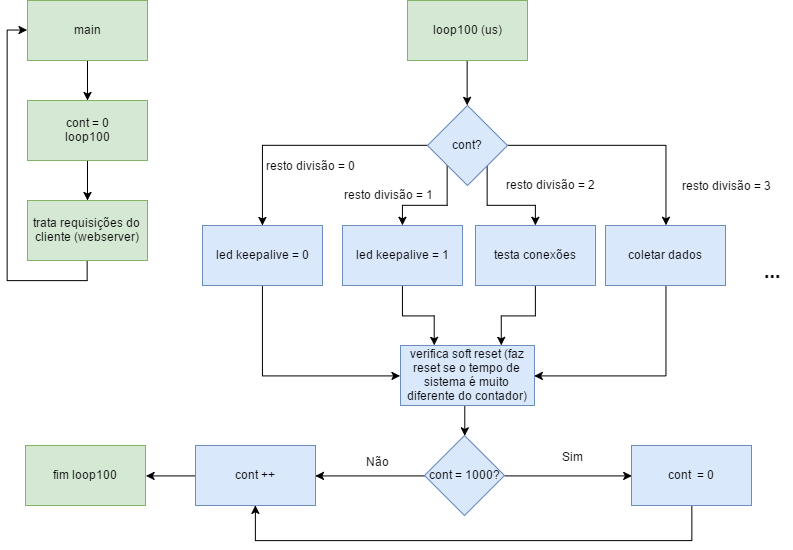
\includegraphics[width=0.8\textwidth]{rotinaMultiplexacao}
\label{fig:rotinaMultiplexacao}
\end{figure}

\subsubsection{Tratamento de indisponibilidade}
Nos casos de indisponibilidade de Internet, servidor ou rede local, o seguinte procedimento foi adotado (observe que a indisponibilidade do próprio módulo é tratada pelo circuito antitravamento):

\begin{figure}[H]
	\centering
	\caption{Tratamento de indisponibilidade de recursos}
  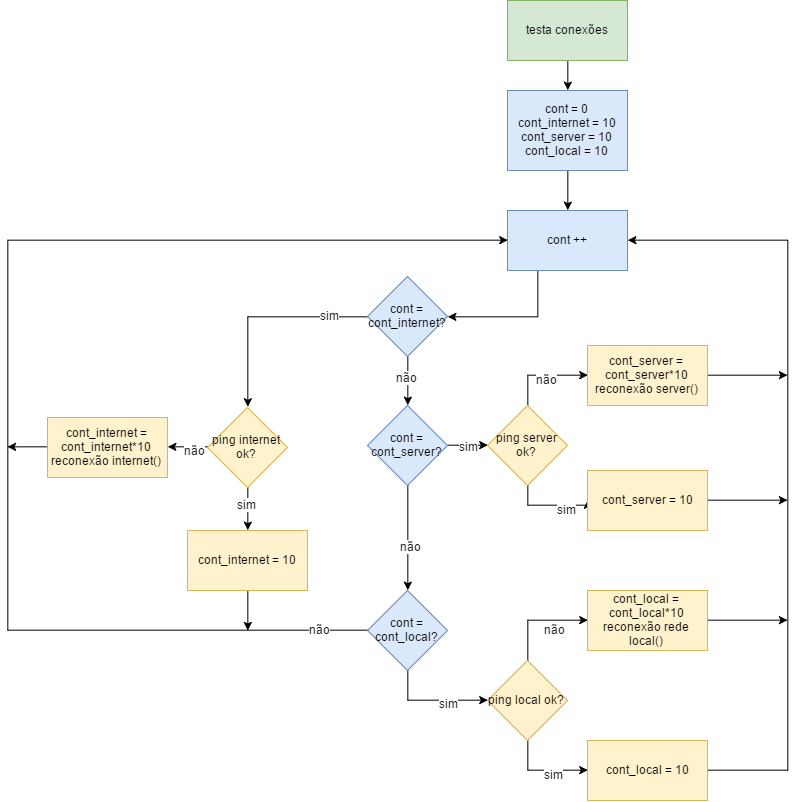
\includegraphics[width=0.8\textwidth]{tratamentoIndisponibilidade}
\label{fig:tratamentoIndisponibilidade}
\end{figure}

Com esse procedimento, as tentativas de reconexão à Internet, servidor e rede local estão segregadas e com tentativas realizadas em intervalos de tempo sucessivamente maiores. Desta forma, conseguimos gerenciar esses procedimentos, já que o nível de processamento é baixo.

\subsubsection{DoS Local (\textit{Evil Twin})}
No caso de ataque de \textit{Evil Twin} - no qual uma rede mal intencionada, usualmente aberta, usa o mesmo SSID da rede original, com o objetivo de obter a senha - o sistema pode ficar indisponível até ao nível local. Módulos podem se conectar à rede mal-intencionada e ficarem somente com as funcionalidades offline, como acionamento de lâmpada por botão físico acoplado ao módulo. Outro problema é a queda da rede por interferência de radio frequência ou outro mecanismo utilizado pelo usuário mal intencionado para que os clientes se desconectem, tentem reconexão e forneçam a senha da rede.

Para mitigar esses riscos, os módulos executam o seguinte procedimento:
\begin{figure}[H]
	\centering
	\caption{Tratamento de ataque de DoS Local}
  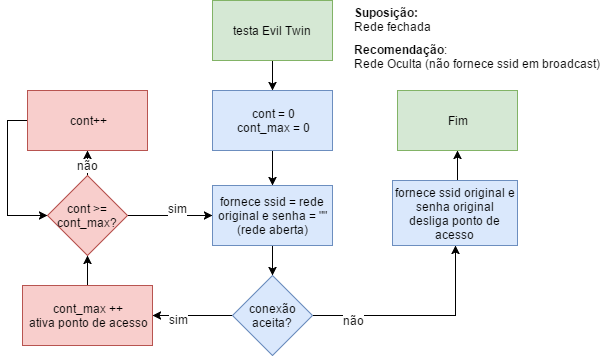
\includegraphics[width=0.8\textwidth]{tratamentoDoS}
\label{fig:tratamentoDoS}
\end{figure}

\subsubsection{Diagrama}
Abaixo está o diagrama do circuito impresso (PCB) feito em conjunto com o Projeto Katz-House\footnote{Katz-House, Fabio Hayashi. Projeto Pessoal, 2017.}. Funcionalidade, componentes e arquitetura foram responsabilidade do Projeto Hedwig, enquanto a disposição física, se atentando para problemas de interferência e mantendo o módulo o menor possível foi responsabilidade do Projeto Katz-House.

\begin{figure}[H]
	\centering
	\caption{Diagrama PCB do Módulo Base}
  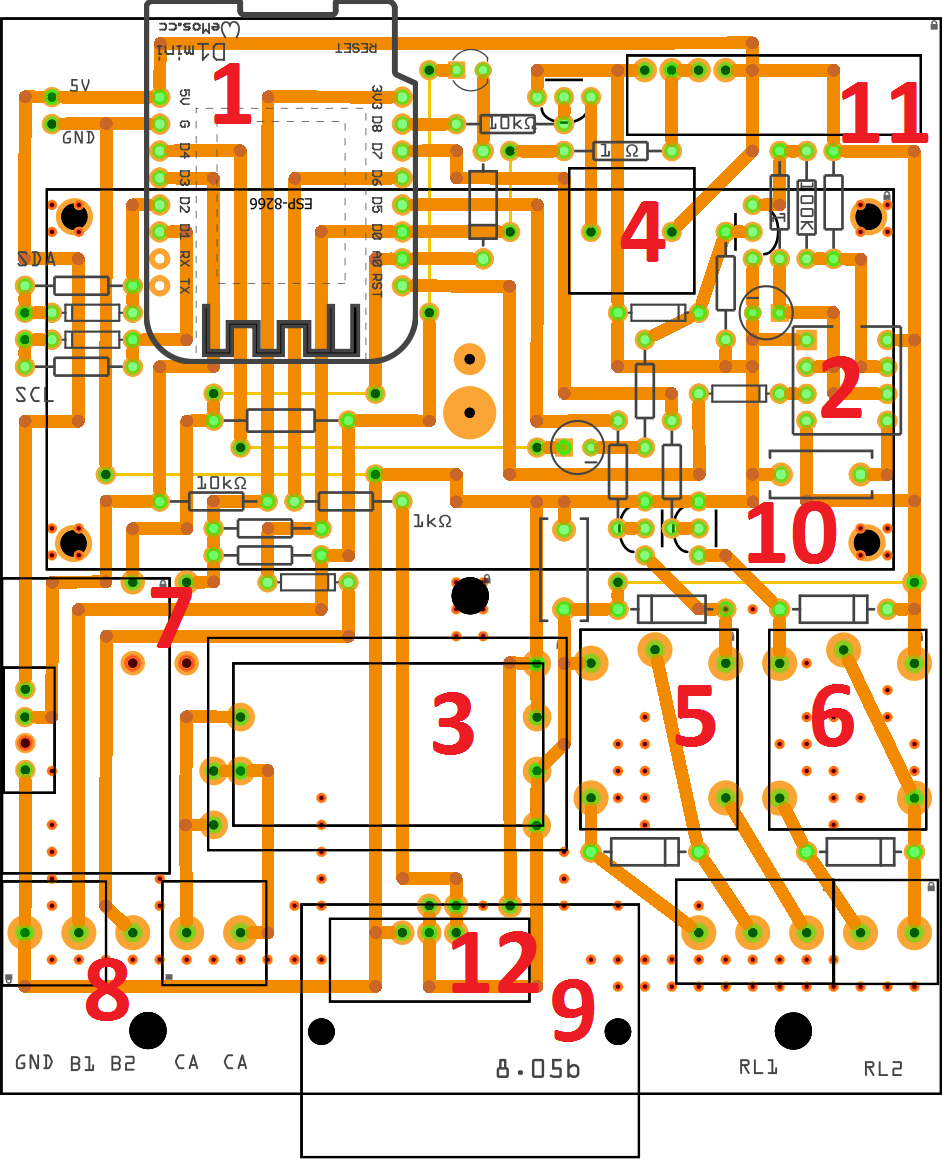
\includegraphics[width=0.8\textwidth]{diagramaModuloBase}
\label{fig:diagramaModuloBase}
\end{figure}

\begin{enumerate}
\item Wemos D1 mini
\item Astável 555
\item Fonte 5V 3W
\item \textit{Buzzer}
\item Relé 1
\item Relé 2
\item Hard Reset
\item Botões
\item Presença
\item RF-RX
\item RF-TX
\end{enumerate}

\begin{figure}[H]
	\centering
	\caption{Diagrama PCB do Módulo Base}
  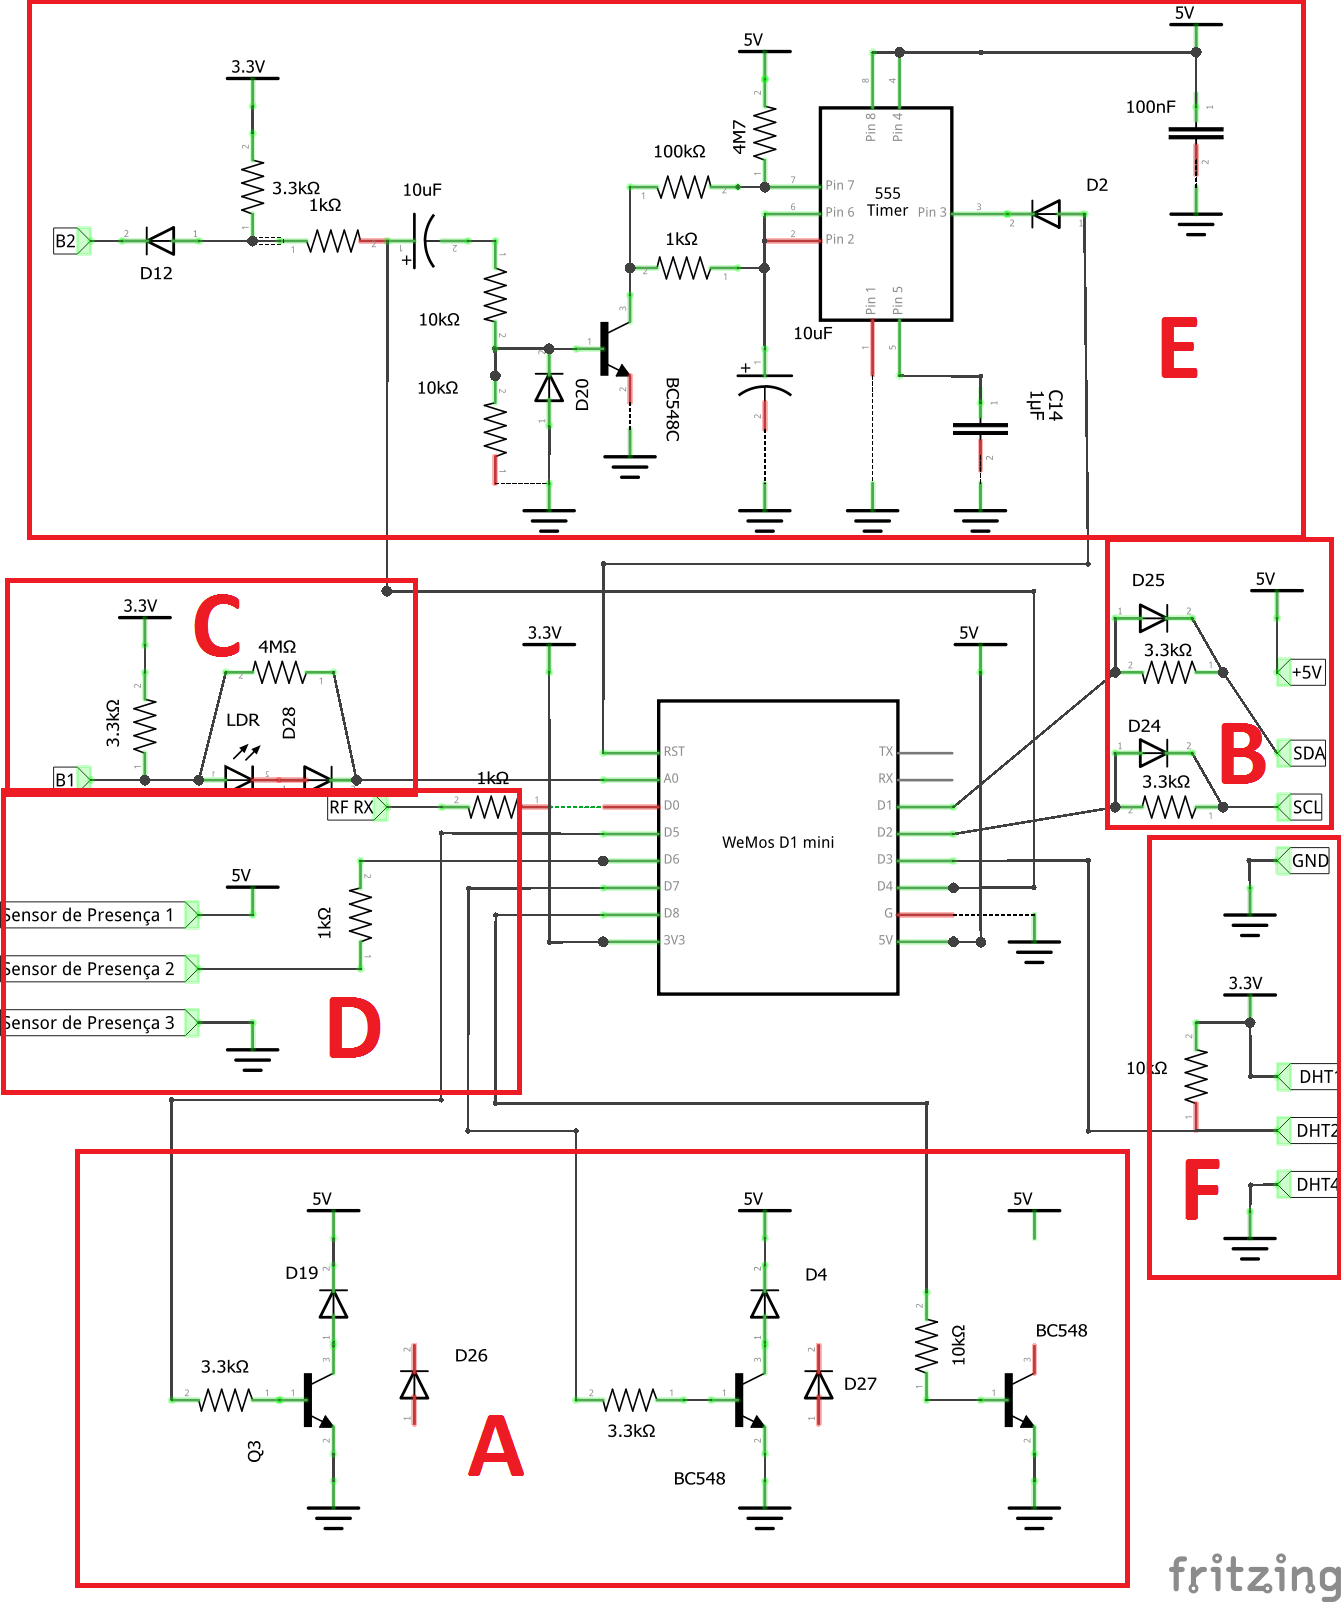
\includegraphics[width=0.8\textwidth]{esquematicoModuloBase}
\label{fig:esquematicoModuloBase}
\end{figure}

\begin{description}
\item [A - Saídas] Circuitos simples de transistor para acionamento de relés (para lâmpadas) e buzzer.
\item [Proteção 3V3 5V] Como o display trabalha com tensão de 5V, há proteções com diodos para não danificar as entradas digitais do Wemos D1 mini, que trabalha com tensão de 3V3.
\item [3 Entradas em A0] O circuito tem como entradas um botão (para acionamento do relé 1), o LDR (para chaveamento do backlight do display), e um outro botão para hard reset do dispositivo, todos numa entrada analógica, cujo mapeamento E/S é da seguinte forma:

\begin{figure}[H]
	\centering
	\caption{Entradas Em A0}
  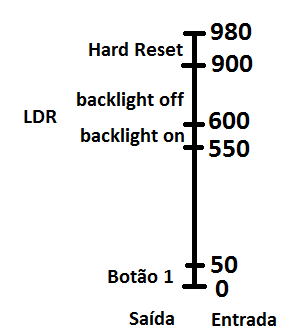
\includegraphics[width=0.4\textwidth]{entradasEmA0}
\label{fig:entradasEmA0}
\end{figure}

\item [Presença ou RF-TX] A entrada digital D6 é usada exclusivamente como entrada do sensor de presença PIR ou receptor RF.
\item [Astável 555 para Hard Reset e Botão] A porta D6 é usada como LED \textit{keep alive} do módulo. Sua demora ao piscar indica que o módulo está travado ou demorando muito para processar algo, o que não deveria acontecer, uma vez que os procedimentos estão multiplexados no tempo, de acordo com seus tempos limite. Dessa forma, conectamos essa saída a um circuito antitravamento, que executa o reset nos casos mencionados, de travamento ou \textit{timeout}.

O primeiro capacitor tem como objetivo desacoplamento DC, de forma que a entrada do circuito envolvendo o astável 555 seja somente AC. Assim, travamentos em 0 ou 1 indicam travamento.

Enquanto o LED pisca em intervalos esperados (regularmente), o transistor conduz e mantém uma saída dente de serra muito próxima de 0. Quando o módulo trava, o transistor não conduz mais, e a saída passa a oscilar entre 1/3 e 2/3 da tensão total (observe que o carregamento é feito pelo resistor de 4M7, muito maior que o resistor de 100k, fazendo com que o tempo de carga seja muito maior que o tempo de descarga, uma vez que esses tempos são diretamente proporcionais à constante de tempo dos circuitos RC, que é dada pelo produto do R*C). Durante a descarga, o reset da placa é realizado. Observe que os tempos foram ajustados pelos valores dos componentes discretos, para que o tempo entre resets sucessivos seja menor que o tempo necessário para o módulo voltar a funcionar após um reset.

Segue abaixo uma ilustração sobre o funcionamento do circuito.

\begin{figure}[H]
	\centering
	\caption{Funcionamento do Circuito de Antitravamento}
  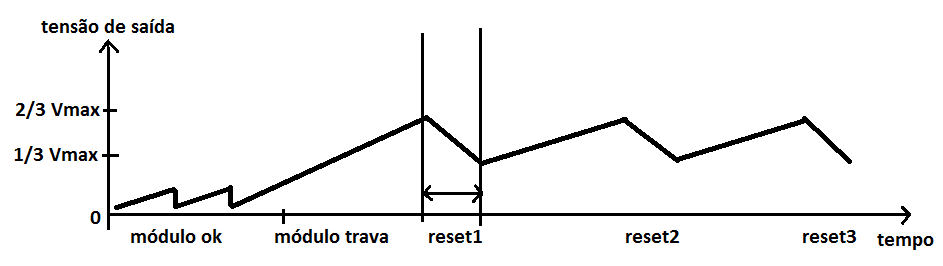
\includegraphics[width=0.8\textwidth]{circuitoAntiTravamento}
\label{fig:circuitoAntiTravamento}
\end{figure}

\item [DHT11] Entrada D3 é ligada a uma montagem básica para leitura de umidade e temperatura através do periférico DHT11.

\end{description}

\subsection{Módulo de Interface com Sistema de Alarmes}
% TODO vai ter essa secao mesmo?

\subsection{Módulo de Acesso}

Buscando garantir mais segurança e comodidade para o acesso à residência, além do controle de abertura, o módulo de acesso atua em paralelo com uma fechadura eletrônica, que é acionada por meio de controle remoto, que utiliza ondas de rádio. Assim, mesmo com falha total do sistema, o usuário pode abrir o portão diretamente, sem a necessidade de acesso à Internet.

\begin{figure}[H]
	\centering
	\caption{Diagrama ilustrativo do módulo de Acesso ao Portão}
  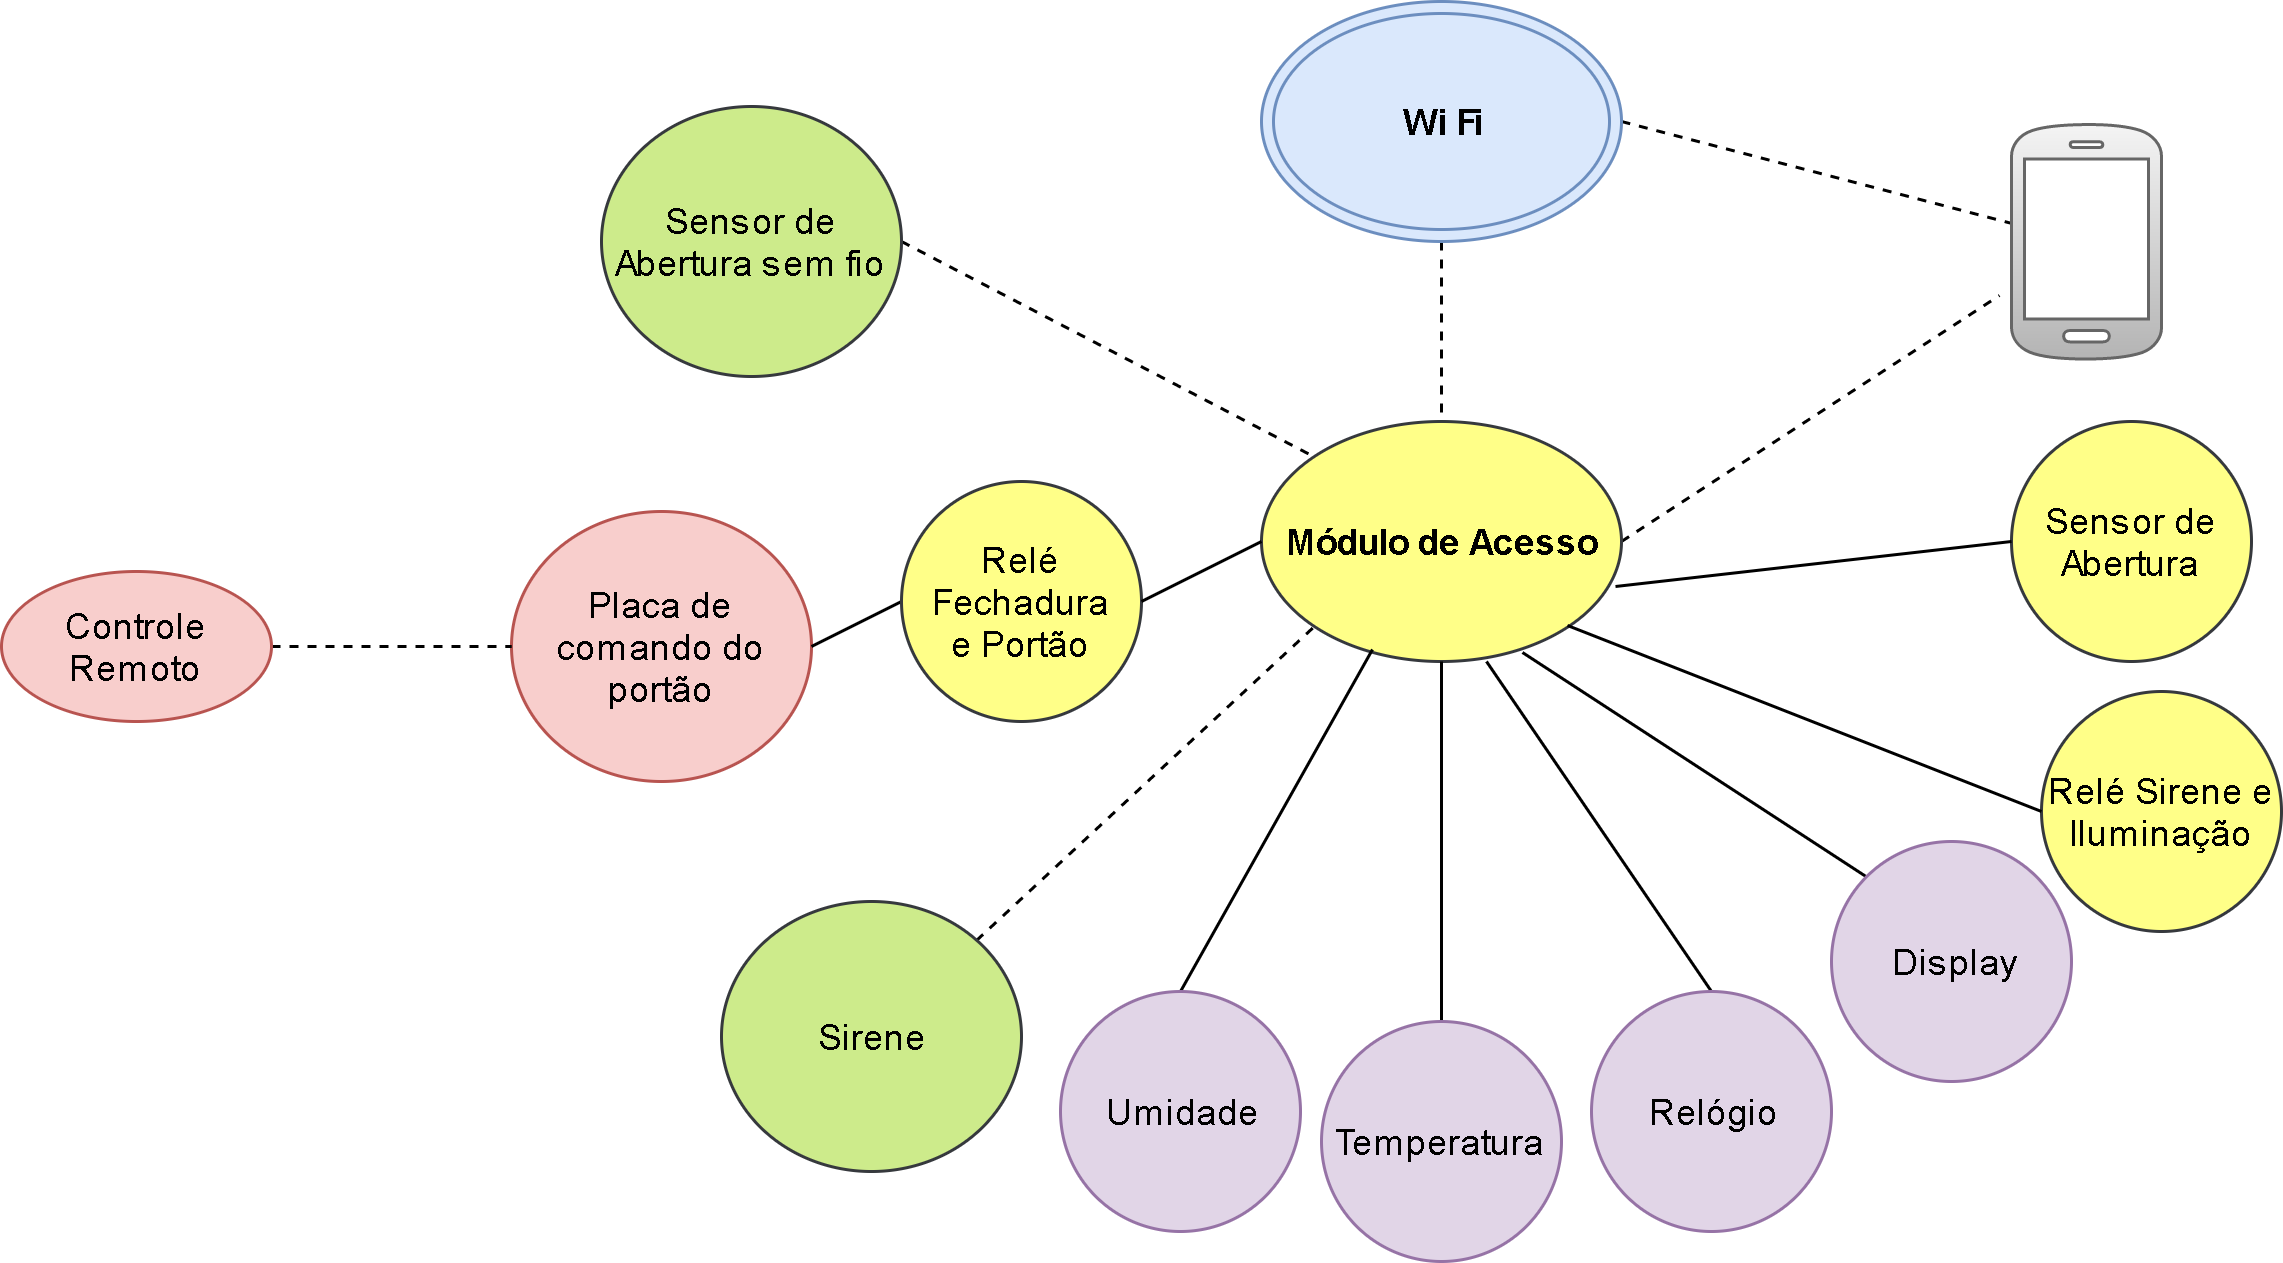
\includegraphics[width=0.8\textwidth]{diagramaModuloAcesso}
\label{fig:diagramaModuloAcesso}
\end{figure}

O diagrama ilustra, em vermelho, os sistemas já existentes. Sensor e sirene sem fio adicionais são mostrados em verde (dispositivos externos ao módulo, que se comunicam por rádio); o próprio módulo de acesso, com um buzzer embutido, e sua conexão com a rede local Wi-Fi ou sua conexão direta com o celular (quando o módulo opera como um ponto de acesso de rede), em amarelo; além de funcionalidades adicionais, em roxo.

A comodidade, no exemplo em questão, está em abrir o portão por meio do celular, ao utilizar o aplicativo web ou o aplicativo local (de emergência), sem a necessidade de carregar uma chave ou controle.

Entretanto, é necessário que a realização do controle de acesso seja feita de maneira segura. Assim, a funcionalidade é apenas local (o usuário deve estar com o celular conectado à rede da casa para acessar a página local), e um algoritmo de rotação de teclas é utilizado, para evitar que pessoas mal intencionadas possam (1) olhar e copiar a senha que o usuário digita em seu celular e (2) copiar os dados de abertura e usá-los mais tarde (\textit{middle man}). Na última alternativa, a cada acesso de um usuário, um novo mapeamento de teclas é gerado e enviado ao usuário. Mesmo que haja cópia, ela não funcionará devido ao mapeamento ter mudado. Observe ainda que a fechadura eletrônica, por si só, já estava vulnerável a este tipo de ataque - há, inclusive, dispositivos copiadores de senhas.

Outro aspecto de segurança é a preocupação dos usuários em esquecer a porta ou portão abertos. Para mitigar esse perigo, o módulo deve monitorar, por meio de um sensor, o estado vigente (aberto/fechado), e alertar localmente (por meio de \textit{buzzer}) e remotamente (e.g. por email ou notificação no \textit{smartphone}) o usuário. Essa e outras configurações (como de rede) são acessadas por uma senha diferente daquela de abertura, de modo que a interface básica seja simples para uso.

Para o caso de falha de envio de notificação (e.g. servidor fora do ar, ou indisponibilidade na conexão), há um algoritmo de novas tentativas com tempos progressivamente maiores conforme as falhas ocorrerem, buscando deixar o módulo disponível para outras funções. Tratamento análogo é realizado no servidor local, e no sistema de mensageria, de modo a evitar perdas de mensagens, mesmo em situações desfavoráveis. Para o caso de falta de conexão à internet, o módulo não seria controlável pela nuvem, com o aplicativo web, mas sim com o aplicativo emergencial, com a ativação do \textit{Access Point}, desenvolvido para operar diretamente com os módulos, sem intermédio do servidor local e dos serviços remotos.

Por meio dos dados de login dos usuários no sistema, é possível saber qual dos usuários que solicitou a abertura do portão. A persistência destes acessos pode ser analisada, e, utilizando-se técnicas de Machine Learning, perfis de acesso podem ser determinados, e evoluir até o sistema saber quando houver um acesso em horário inesperado e notificar o usuário remotamente. O aprendizado de máquina é fundamental aqui para descobrir comportamentos que podem ser entendidos como suspeitos. Para um usuário que costuma chegar em um horário aproximado todos os dias, e acionar funções semelhantes da casa, uma tentativa de acesso que não se enquadre em tais padrões pode ser produto de atividade criminosa, a qual pode ser informada pela casa para uma central, que acionaria a polícia caso não seja um falso positivo.

%\subsection{Módulo de Quarto}
% TODO

%\subsection{Módulo de Aquário}
% TODO

%\subsection{Módulo de Cozinha}
% TODO
